\ifdefined\included
\else
\setcounter{chapter}{3} %% Numéro du chapitre précédent ;)
\dominitoc
\faketableofcontents
\fi

\chapter{Searching for a route with semantic knowledge}
\chaptermark{Searching for a route with an ontology}
\label{chap:3}
\minitoc

The contribution presented in this chapter is excerpted from our work, published in the proceedings of the Spatial Language Understanding (SpLU) 2019 workshop~\cite{sarthou_2019_semantic}. In this manuscript, the contribution is more detailed and discussed. This work is part of the MuMMER project, aiming at developing a robot guide in a mall. At the end of this thesis, a chapter is dedicated to the presentation of the project and the integration of the current contribution is a robotic system.

\section{Introduction}

We all have already been requested, or have ourselves request, for a route toward public space in a city, a shop in a shopping centre, or more simply a toilet in a house. When providing such information to a lost person we perform what is commonly called a guidance task. Even if it can seem evident for us, developing a robot able to perform it can be challenging. In this chapter, we choose to focus on the sub-task consisting to generate the explanation sentence. This sub-task is called the route description. To perform it, we first need a set of knowledge about the environment in which the guided person will walk, such as the paths, the intersections of the paths, or the elements alongside them. Then, we need a set of "good practices" to provide a route easy enough to follow and to remember.

In the Human-Robot Interaction (HRI) field, robots guides have been study intensively and deployed into shopping centers~\cite{okuno_2009_providing}, museums~\cite{burgard_1999_museum, clodic_2006_rackham, siegwart_2003_robox}, or airport~\cite{triebel_2016_spencer}. From a knowledge representation point of view, we can notice the use of metrical representations~\cite{thrun_2007_simultaneous} or topological representations~\cite{morales_2011_modeling} to represent the environment in which the robot evolves. Since we focus on the route description task, we consider that the robot does not accompany the human to his final destination but rather explains how to reach it. Consequently, the metrical representation will not be considered as being mainly used for navigation purpose~\cite{thrun_2007_simultaneous}. To perform more specifically a route description, topological knowledge is not sufficient. In addition to the topology of the environment, the robot needs to know the types of the elements composing the environment and their names in natural language. Some contributions have thus try to mix metrical or topological representations with semantic ones to hold this additional knowledge~\cite {satake_2015_should, chrastil_2014_cognitive, zender_2008_conceptual}. However, mixing them can create a lack of uniformity among the overall knowledge representation. In this way, creating a unique representation allowing a robot to compute routes and expressing them could ensure uniformity among the knowledge.

Even having a rich enough representation of its environment, the robot has to find a route not for it but for the guided human. A robot accompanying the human only has to determine a path, adapted to its capacities and interpretable only by it. Providing a route to a human, the route has to be adapted to the human capabilities. For example, in an outdoor environment, we will not give the same route for a car driver or a cyclist. In the context of a mall, we will not give a route with stairs along to a mobility-impaired person or to someone with a shopping cart. Once an adapted route computed, the robot has to explain it. Where interactive maps only have to highlight a path, here, the robot has to generate a sentence that the human will memorize. For sure the robot will not instruct a human with a sentence like "walk 30 meters them turn -90 degrees". This would not be adapted. The use of orientation and reference to elements of the environment will be needed through a sentence like "walk until the florist then turn left".

The first contribution of this chapter is a \textbf{unified representation} of an indoor environment using an ontology, to include both topological and semantic knowledge. Then, on the basis of this representation, we propose a first algorithm to \textbf{find a suitable route} to be explained to a human and a second algorithm to \textbf{verbalize a route} in an appropriate way.

%concerning semantic representation of indoor environment and
First, we review the literature of route description. Then, we introduce the reader to our unified semantic representation under the name of Semantic Spatial Representation (SSR). We then present the algorithm used to compute the route and in a second time the algorithm to verbalize the previously computed route. We end this chapter with experimental results on both emulated and real environments.

\section[Related work]{Related work: describing a route}

%\subsection{Describing a route}

In the literature, a route description task is defined as being a particular kind of spatial description. First, from a cognitivist point of view, Denis in~\cite{denis_1997_description} has identified three main cognitive operations used to generate such a spatial discourse: 1) the activation of an internal representation of the environment, 2) the planning of a route in this representation, 3) and finally the formulation of the procedure to follow. From a computer science point of view, Cassell in~\cite{cassell_2007_trading} view the second operation as the fact of finding a set of routes segment, each connecting two important points, and the third operation as chronologically explaining the route segments. In the same way, Mallot in~\cite{mallot_2009_embodied}, see the second operation as the fact of selecting a sequence of places leading to the objective, and the third as managing declarative knowledge to choose the right action to explain at each point of the sequence. While both second operations are equivalent, the thirds about the formulation of the procedure are rather complementary.

The route description task has been extensively studied through verbal and textual communication to understand how humans communicate spatial knowledge. The goal of such studies has been to identify the invariants but also the good practices ensuring the success of the task. Through five experiments in both urban and interior environments, Allen is~\cite{allen_2000_principles} has identified three basic practices seen as being important for communicating knowledge about routes. They can be summarized as follows: a) respect the spatiotemporal order, b) concentrate on the information about the points of choice and c) use landmarks that the listener can easily identify.

This latter practice about the use of landmarks, also called reference marks, has been identified by Tversky in~\cite{tversky_1999_pictorial} has been critical information for the success of a route description. With his anterior contribution~\cite{tversky_1998_space}, he finds that in addition to information about actions, reorientation, and direction, 91\% of the guidance instructions contains the use of landmarks. These results trend at confirming the ones of Denis in~\cite{denis_1997_description}. In an anterior study, Montello in~\cite{montello_1993_scale} tries to identify when the use of landmarks appear in a description. Defining the \textit{Vista} space as being the area within sight and the \textit{Environmental} as being the rest of the environment reachable through locomotion, he finds that guides usually used landmarks when the target places were no longer in the \textit{Vista} space but in the \textit{Environmental} one. Moreover, with regard to~\cite{tversky_1999_pictorial}, the use of landmark more precisely appears during an explanation of a direction changing. In addition, their choice is based on salient features over a route description~\cite{nothegger_2004_selection}.

\begin{figure}[ht!]
\centering
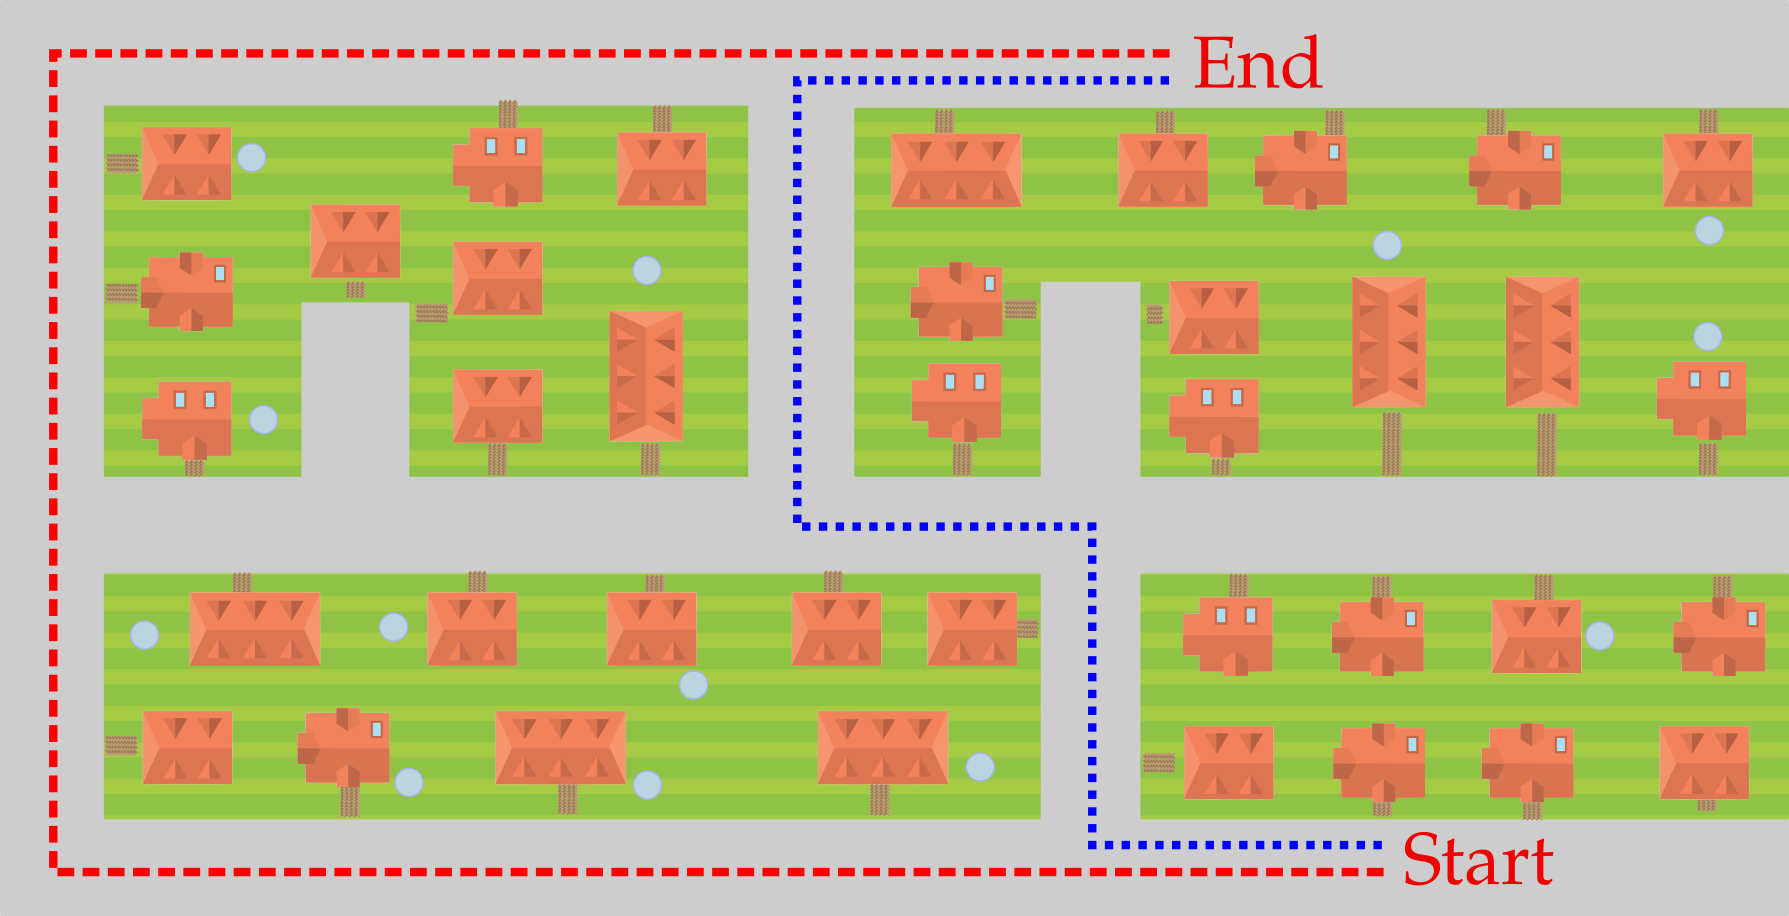
\includegraphics[scale=0.22]{figures/chapter3/landscape/landscape.png}
\caption{\label{fig:chap3_shortest} Comparison of two routes in terms of complexity and length. Even if the blue route (. . .) is the shortest many directions changing are required. Each of them is a risk for the guided person to make a mistake and be lost again. The red route (- - -), although being a bit longer, is easier to explain and to remember, and has few directions changing.}
\end{figure}

Even if the use of landmarks helps at understanding direction changing by anchoring the action to be performed, they still are a risk for the guided person to make a mistake, taking the wrong path. Where the length of the route would be an important criterion is the choice of a route, its complexity is also to be taken into account when we need to explain it. Morales in~\cite{morales_2015_building} argued that reducing the route complexity, in terms of the number of stages composing it, should be prefered to its length. This feature reduces the risk of mistake concerning the choice to make along it and also has an impact on its understanding and memorization. This criteria of minimal explanation can be compared to the Grice's Maxim of quality~\cite{grice_1975_logic}. In the example of figure~\ref{fig:chap3_shortest}, some should prefer to explain the red route rather than the blue one, even if it is longer.

Finally, to explain the same route Taylor in~\cite{taylor_1992_spatial} has noticed that a speaker can use two kinds of perspective. First, the \textit{survey} perspective trend at adopting a bird's eye view point of the environment, meaning a top view of it like as looking at a map. With this perspective, the speaker refers to the different landmarks of the route with respect to one another. They are thus referred to using terms including north-south-east-west. This perspective is opposite to the \textit{route} perspective. With such a perspective, the speaker mentally navigates along the route, making an imaginary tour of the environment. As a result, he refers to the landmarks with respect to the future guided person position along the route. The landmarks are thus referred to using terms like left, right, front, or back. In~\cite{taylor_1996_perspective}, they notice that the survey perspective is generally used for open environments whereas the route perspective is generally used in environments with already identified paths. For indoor environments, the latter should thus be preferred to facilitate route understanding and memorization.

%\subsection{Environment represention to compute routes}

%Regarding the environment representation generally used to find itineraries, we can first take a look at GNSS road navigation systems. In \cite{liu_1997_route} or \cite{cao_2009_gps}, we find the same principle of a topological network representing the roads with semantic information attached to each of them. Such representation seems adapted regarding the performance required for such systems operating in very large areas. However, GNSS road navigation systems must respond only to this unique task of finding a route where a robot is expected to be able to answer various tasks and unprecise destination request. For our application, we thus need a representation that can be used more widely while still allowing the search for routes.

%Satake in~\cite{satake_2015_field} has developed a topological graph for the route search process. To understand the human request about the destination node in the graph, they build an ontology, providing a semantic description of them. The description informs about the places types (e.g. cloth shop, restaurant, ...), names and nickname, and the sold items. However, as explained in~\cite{morales_2015_building}, such a map with annotated elements does not provide a suitable base to generate route explanations using a route perspective. Nevertheless, we can note that the use of an ontology, if suitable to describe the meaning of the elements of the environment. In the same way, you can also describe other elements than shops, like stairs, elevator, entrance, or escalator. To unify the representations, we could thus, represent the topology in an ontology. Since both are graphs, this representation should be feasible and provide more information about the elements along the paths.

%To semantically represent an environment, Kuipers in~\cite{kuipers_2000_spatial} introduce the Spatial Semantic Hierarchy (SSH). With it, he defines a 'topological level' composed of three main elements being the places, paths, and regions, as well as relations between them. To create our semantic description of an indoor environment, we thus choose to take it as a basis. The concepts definition will be refined in the next section.

%Since this contribution is focused on a pattern to describe environment and algorithms using it the compute routes, the presented representation are made by hand. However, many contributions trend to automatically generate a topological graphs from geometric measurements (e.g. Region Adjacency Graphs \cite{kuipers_2004_local}, Cell and Portal Graphs \cite{lefebvre_2003_automatic}, hierarchical models \cite{lorenz_2006_hybrid}, or from natural language \cite{hemachandra_2014_learning}). Even if we do not have used such techniques for the moment, our contribution could benefit from these works, solving the complexity of creating such a representation by hand.

\section{The Semantic Spatial Representation}

Satake in~\cite{satake_2015_field} has developed a topological graph for the route search process. To understand the human request about the destination node in the graph, they build an ontology, providing a semantic description of them. The description informs about the places types (e.g. cloth shop, restaurant, ...), names and nickname, and the sold items. However, as explained in~\cite{morales_2015_building}, such a map with annotated elements does not provide a suitable base to generate route explanations using a route perspective. Nevertheless, we can note that the use of an ontology, if suitable to describe the meaning of the elements of the environment. In the same way, you can also describe other elements than shops, like stairs, elevator, entrance, or escalator. To unify the representations, we could thus, represent the topology in an ontology. Since both are graphs, this representation should be feasible and provide more information about the elements along the paths. As explained in the previous chapters of this thesis, ontologies are widely used for knowledge representation, to capture the meaning of the elements of an environment but also to encode knowledge dedicated to the robot's internal process. In this way, they provide a good interface between the robot's process and its human partner in terms of interaction.% Where Satake~\cite{satake_2015_field} already use an ontology to describe the different shops of a shopping center, in this section, a present how to represent the topology of the environment in addition.

To semantically represent an environment, Kuipers in~\cite{kuipers_2000_spatial} introduce the Spatial Semantic Hierarchy (SSH). With it, he defines a 'topological level' composed of three main elements being the places, paths, and regions, as well as relations between them. To create our semantic description of an indoor environment, we thus choose to take it as a basis. However, this representation does not use an ontology, we thus present how we extend it to represent the topology in an ontology. The resulting representation and its underline pattern are what we called the Semantic Spatial Representation (SSR).

Since this contribution is focused on a pattern to describe environment and algorithms using it the compute routes, the presented representation are made by hand. However, many contributions trend to automatically generate a topological graphs from geometric measurements (e.g. Region Adjacency Graphs \cite{kuipers_2004_local}, Cell and Portal Graphs \cite{lefebvre_2003_automatic}, hierarchical models \cite{lorenz_2006_hybrid}, or from natural language \cite{hemachandra_2014_learning}). Even if we do not have used such techniques for the moment, our contribution could benefit from these works, solving the complexity of creating such a representation by hand.

\subsection{The SSR classes}

Kuipers has defined three distinct concepts being the \textbf{region}, the \textbf{path}, and the \textbf{place}. To represent the topology, we have refined the concepts of place and path. Here bellow, we define these concepts and their refinement. The resulting class hierarchy is representing with the partial TBox of figure~\ref{fig:chap3_tbox}.

\begin{figure}[ht!]
\centering
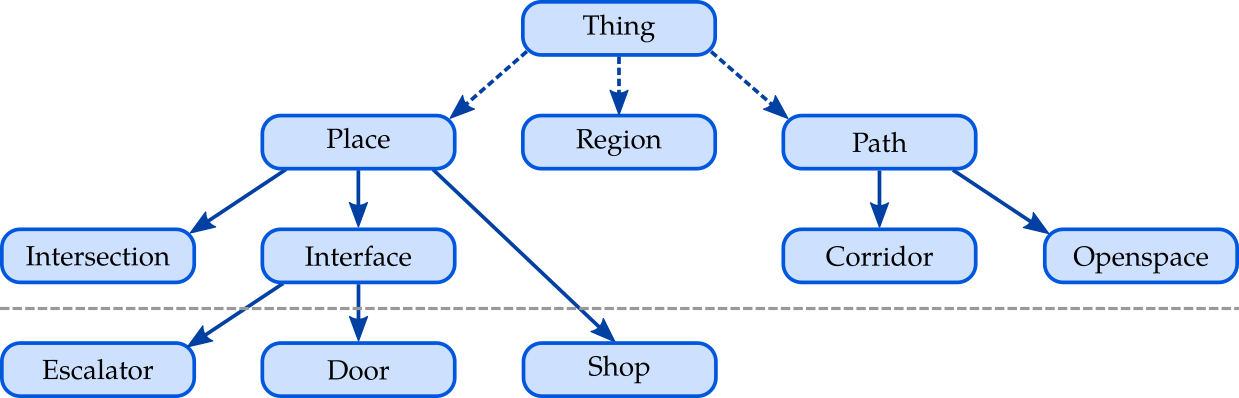
\includegraphics[scale=0.4]{figures/chapter3/ssr_tbox.png}
\caption{\label{fig:chap3_tbox} Representation fo the TBox (classes hierarchy) of the Semantic Spatial Representation used to describe the topology of an indoor environment. While the top part is inherent to the SSR, the bottom one extends the latter to provide more granularity.}
\end{figure}

\paragraph{Region:} It represents a two-dimensional element, drawing an area. An area is a subset of an overall environment. A description of an environment must include at least one region being the entire environment itself. However, defining multiple regions aims at creating a finer representation. For example, for multi-storey buildings, we will at least represent each floor by a distinct region. Regions can be described as being nested if needed.

\paragraph{Path:} It is a one-dimensional element, drawing a line. We can materialize it as an element along which it is possible to move by following it. Even if it is not directly semantically represented, a path must have a direction in order to describe other elements in relation to it. A path can be refined into:

\begin{itemize}
  \item \textbf{Corridor:} It represents a kind of path having a distinct beginning and end. In this way, a corridor cannot be a loop. The direction of the corridor can be chosen arbitrarily. However, its direction defines the position of its beginning and end. Consequently, it also defines the right and left of the corridor. The direction does not mean that the corridor can be use in a unique way but will be used to describe the elements along with it.
  \item \textbf{Open space:} It is a kind of path which does not have any defined begin or end. It thus forms a loop. It can also be viewed as a "potato-shaped" describing the outline of open space. It materializes the possibility of turning the gaze around the room and the fact of not having to go through a defined path to reach one of its points. In a building, a hall would typically be described with such a path.
\end{itemize}

\paragraph{Place:} It represents a point of zero dimension\footnote{For sure it has a 3D location, but here we are speaking of its shape.}. It can either represent a physical or symbolic element. In the context of a mall description, a shop would inherit the place class as a point representing its door can be sufficient to describe it. To represent the topology, we refine it into:
  
\begin{itemize}
  \item \textbf{Path intersection:} It represents the connection between two and only two paths. It is thus a waypoint to go from one path to another. In the case of a crossing between three paths, three intersections have to be described.
  \item \textbf{Interface:} It represents the connection between two and only two regions. It is thus a waypoint to move from one region to another. It can be physical, like a door or a staircase, or symbolic like a passage.
\end{itemize}

To better catch the difference between paths and places, it can be related to the differences between the types of rooms made by~\cite{andresen_2016_wayfinding}. Some rooms in a building such as a house have the main use to circulate from a room to another, they are corridors. Other room, have an explicit use that is not the traffic, they are places even if you can move in.

\subsection{The SSR properties}

The relations introduced by Kuipers aim at representing the connections of places and paths, the order of the places along a path, and the membership of regions. The main relations are the follow:

\begin{align*}
&on(place,path) && place \text{ is on } path \\
&order(path,place1,place2,dir) && \text{the order on } path \text{ from } place1 \text{ to } place2 \text{ is } dir \\
&right\_of(path,dir,region) && path \text{, facing direction } dir \text{, has } region \text{on its right}\\
&left\_of(path,dir,region) && path \text{, facing direction } dir \text{, has } region \text{on its left} \\
&in(place,region) && place \text{ is in } region
\end{align*}

Through these relations, we can first see a slight difference in our use of the main elements. The regions used to group a set of places along a path avoiding in this way to describe each individual place as being at the right/left of a path. Our use of the concept of region will thus require more description for each place but has the advantage to give a finer granularity of huge environment representation with a first level of abstraction. With it, we could imagine a short prior description like "it is on the first floor".

A major limitation of these relations is that they cannot be used in an ontology as they are not all in the form of triplets. The issue comes from the need for a direction de determine the order and the side positions. The properties we introduce aim at fixing this issue and give a more precise description. For example, with their representation, we cannot have a place at the edge of a path. All the properties presented here can be extended with their inverse (e.g. $isIn$ and $hasIn$) for a more expressive model and thus easier handling. The resulting property hierarchy is representing with the partial RBox of figure~\ref{fig:chap3_rbox} 

\begin{figure}[ht!]
\centering
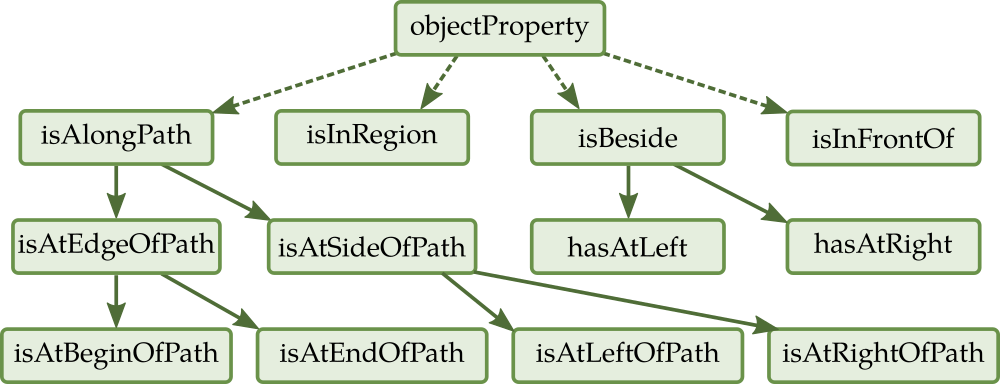
\includegraphics[scale=0.4]{figures/chapter3/ssr_rbox.png}
\caption{\label{fig:chap3_rbox} Representation fo the RBox (properties hierarchy) of the Semantic Spatial Representation used to describe the topology of an indoor environment.}
\end{figure}

\paragraph{isInRegion:} $isInRegion(path/place,\ region)$ describes the fact that a $path$ or a $place$ is in a $region$.

\paragraph{isAlongPath:} $isAlongPath(place,\ path)$ describes the fact that a $place$ is along $path$. Depending if the path is a corridor or an openspace, a finer description can be needed:
\begin{itemize}
  
  \item $isAlong(place,\ corridor)$: Since a corridor is a line, the places along the path can first be described as being either on a side of the corridor with the property $isAtSideOfPath$ or at the edge with the property $isAtEdgeOfPath$. Thanks to direction of the corridor, these properties can be refine with $isAtBeginOfPath$ and $isAtEndOfPath$ for the places at an edge, and  $isAtRightOfPath$ and $isAtLeftOfPath$ for the places at side of the corridor. Even if the direction of the corridor is not directly represented in the ontology, since the places have been position regarding it, we can retrieve it.
  \item $isAlong(place,\ openspace)$: For open spaces, since they do not have beginning or end, places are only defined as being along with an open space.
\end{itemize}

\paragraph{isBeside:} $isBeside(place1,place2)$ describes the fact that $place1$ is beside $place2$. To really represente their order, we use the properties $isAtLeftOf$ and $isAtRightOf$. The choice of these properties is made by positioning themselves at the place and facing the path the place is along.

\paragraph{isInfrontOf:} $isInfrontOf(place1,place2)$ describes the fact that $place1$ is in front of $place2$. This property is not mandatory for all the places but provides a finer description. The more it is used, the more the verbalization of the itinerary will be easy. We will see in the sentence generation section that it is however important to always define a place in front of an intersection. This information will be used to determine if the guided human will have to go left or right in some cases. If there is no described place in front of an intersection, we can use a $emptyPlace$ class that would inherit the $place$ class.

To simplify the description few axioms are made. The property $isInfrontOf$ is sets reflexive. The properties $isAtRightOf$ and $isAtLeftOf$ are set inverse from one another. Finally the chain axiom $isAlong \bullet isIn \rightarrow isIn$ is used to not have to set the $isIn$ property to each place. It can be deduced thanks to the path they are along.

\subsection{An example of description}

\section{Finding routes to the right destination: A two-level search}

\subsection{The region-level: Trim down the search}

\begin{figure}[ht!]
\centering
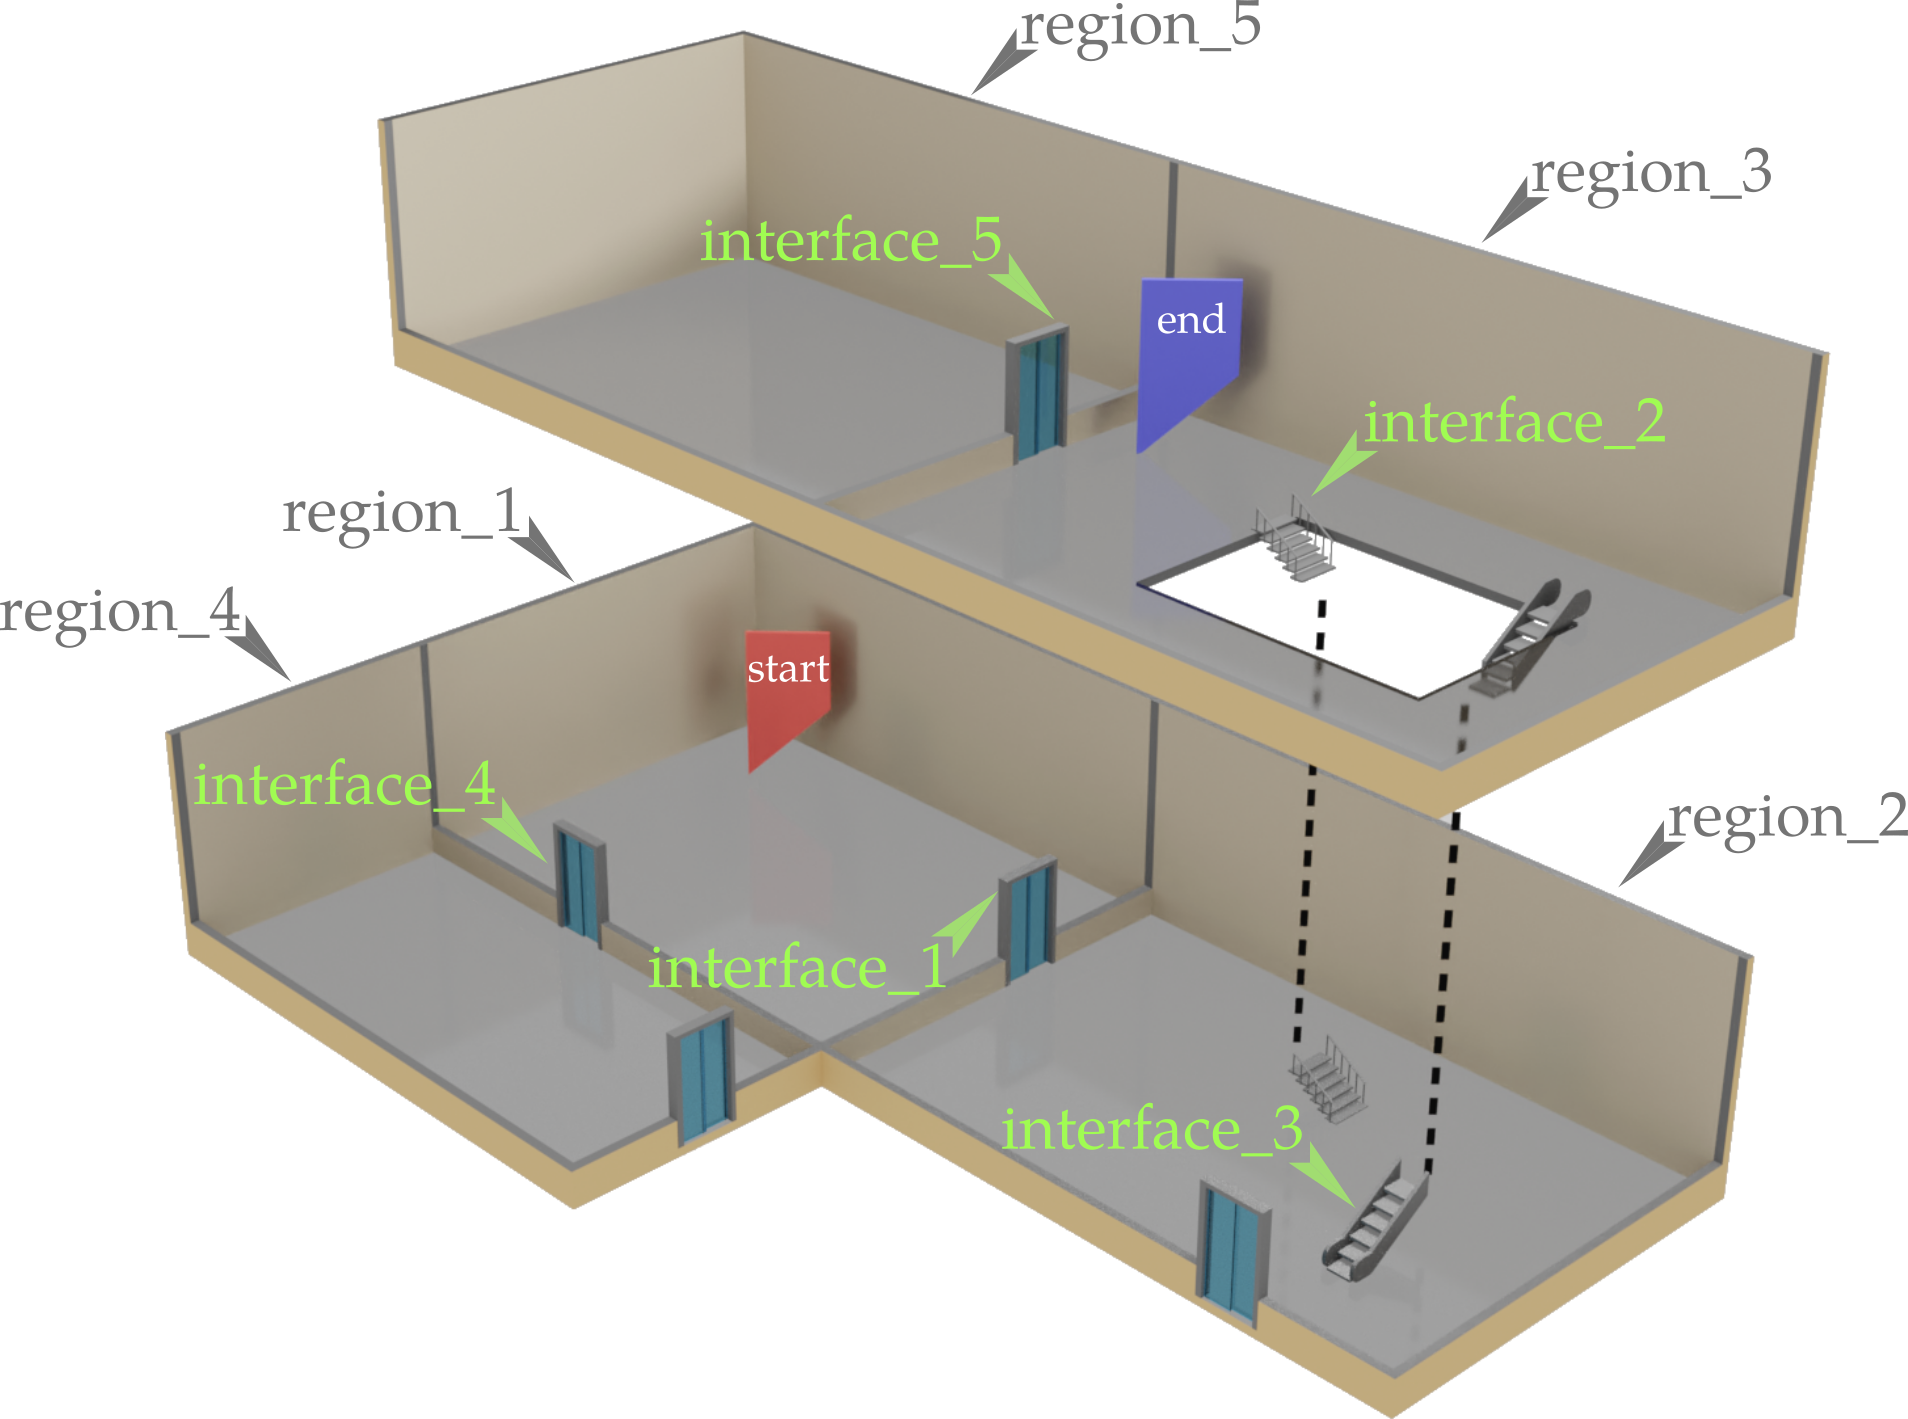
\includegraphics[scale=0.22]{figures/chapter3/building_regions.png}
\caption{\label{fig:chap3_regions} Representation of an environment at the region-level. Regions are linked trhough interfaces. We know that the starting point of the search is in \textit{region\_1} and the goal place is in \textit{region\_3}. }
\end{figure}


\subsection{The place-level: Refine the search}

\begin{figure}[ht!]
\centering
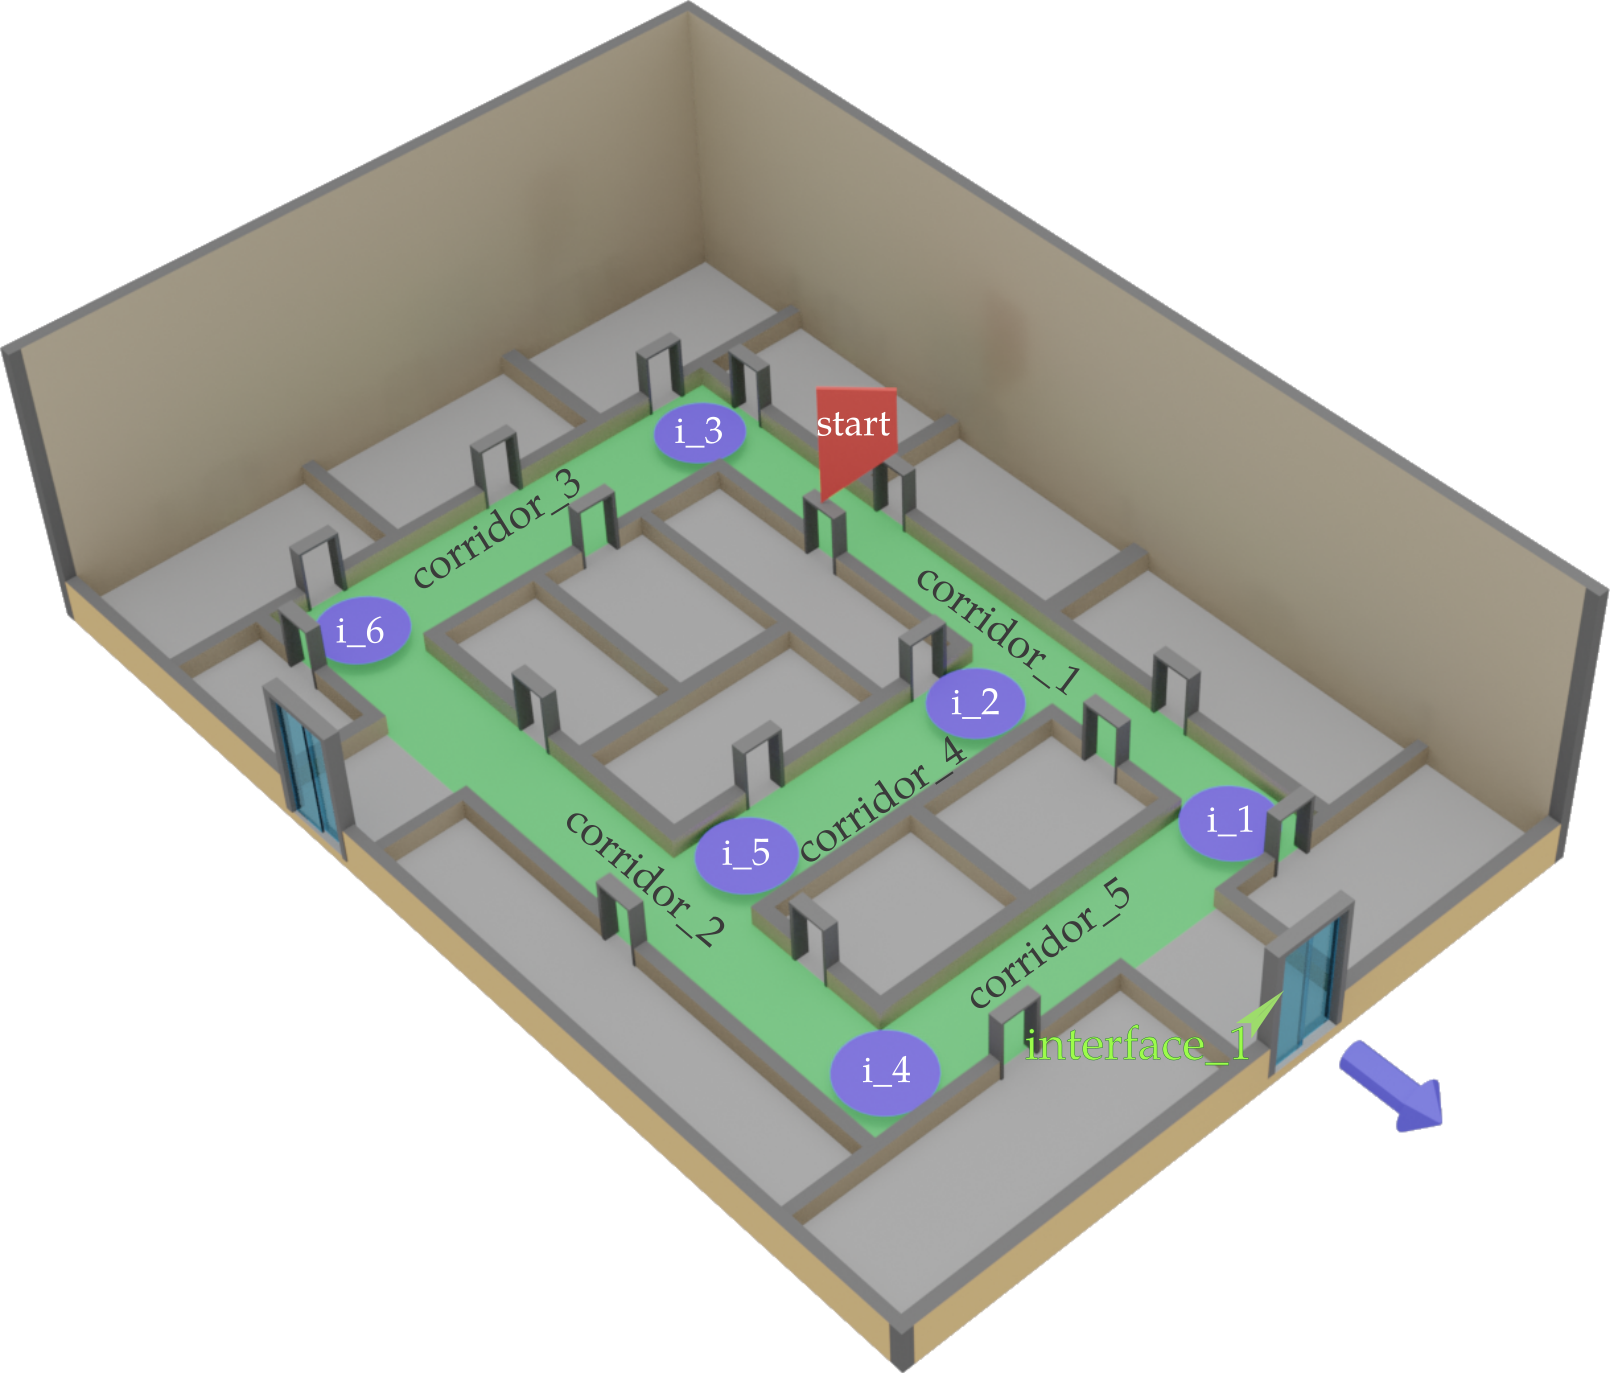
\includegraphics[scale=0.28]{figures/chapter3/region1.png}
\caption{\label{fig:chap3_region1} Representation the \textit{region\_1} at the place-level. A region is composed of paths (here corridors only) connected through intersections. We know that the starting point of the search is along \textit{corridor\_1} and the local goal place is in \textit{corridor\_5}. }
\end{figure}

\subsection{Selecting the most suitable route}

\section{Genarating an explanation in natural language}

\subsection{Putting the robot in your shoes}

\subsection{A pattern-based generation}

\section{Experiment in emulated and real environment}



